\begin{figure}[ht]
  \section{Heatbed}
\adjustbox{valign=t}{\begin{minipage}[t]{0.30\textwidth}
\begin{framed}
  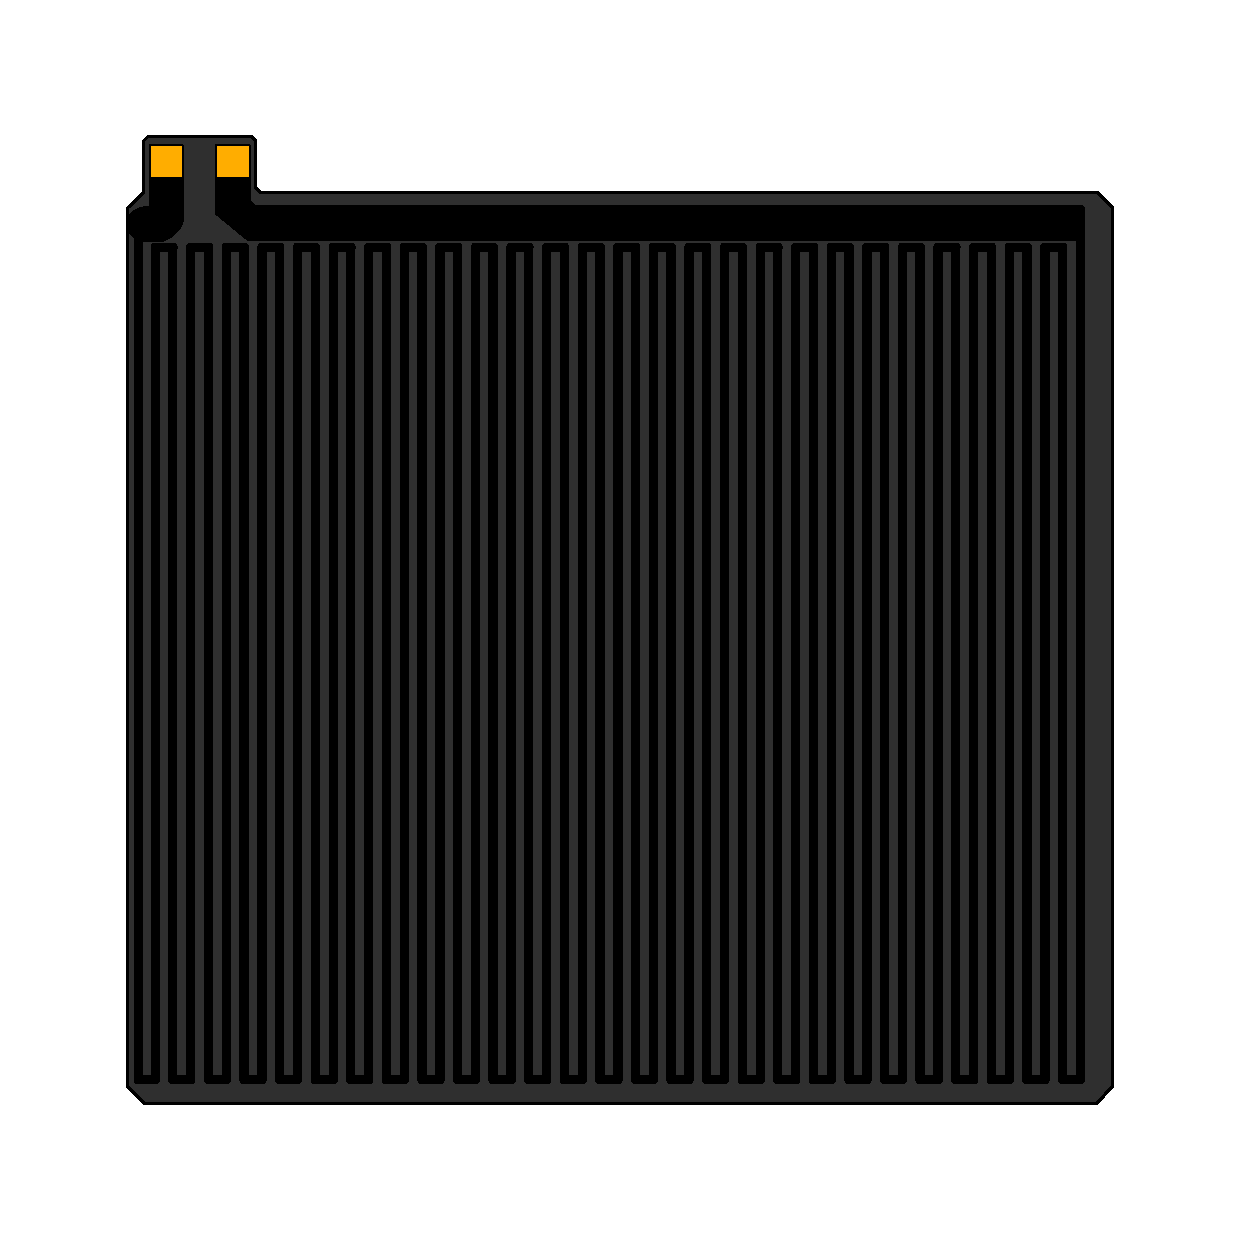
\includegraphics[width=1.0\textwidth, trim = 50px 50px 50px 50px, clip]{./bilder/MK3Bed.pdf}
\end{framed}

\end{minipage}}
% \hfill
\adjustbox{valign=t}{\begin{minipage}[t]{0.60\textwidth}
\vspace{0pt}
\subsection{MK2/MK3 und ähnliche}
\huge
Die meisten PCB / ALU - Heatbed haben eine einzelne Heizschleife. Deshalb konzentriert sich die Wärme in der Mitte und fällt gegen den Rand ab.
% \caption{Kapazität}
\end{minipage}}
% \end{figure}
% \vspace{0.5cm} % ----------------------------------- vspace
% \begin{figure}[ht]
\adjustbox{valign=t}{\begin{minipage}[t]{0.30\textwidth}
% \vspace{0.5cm}
\begin{framed}
  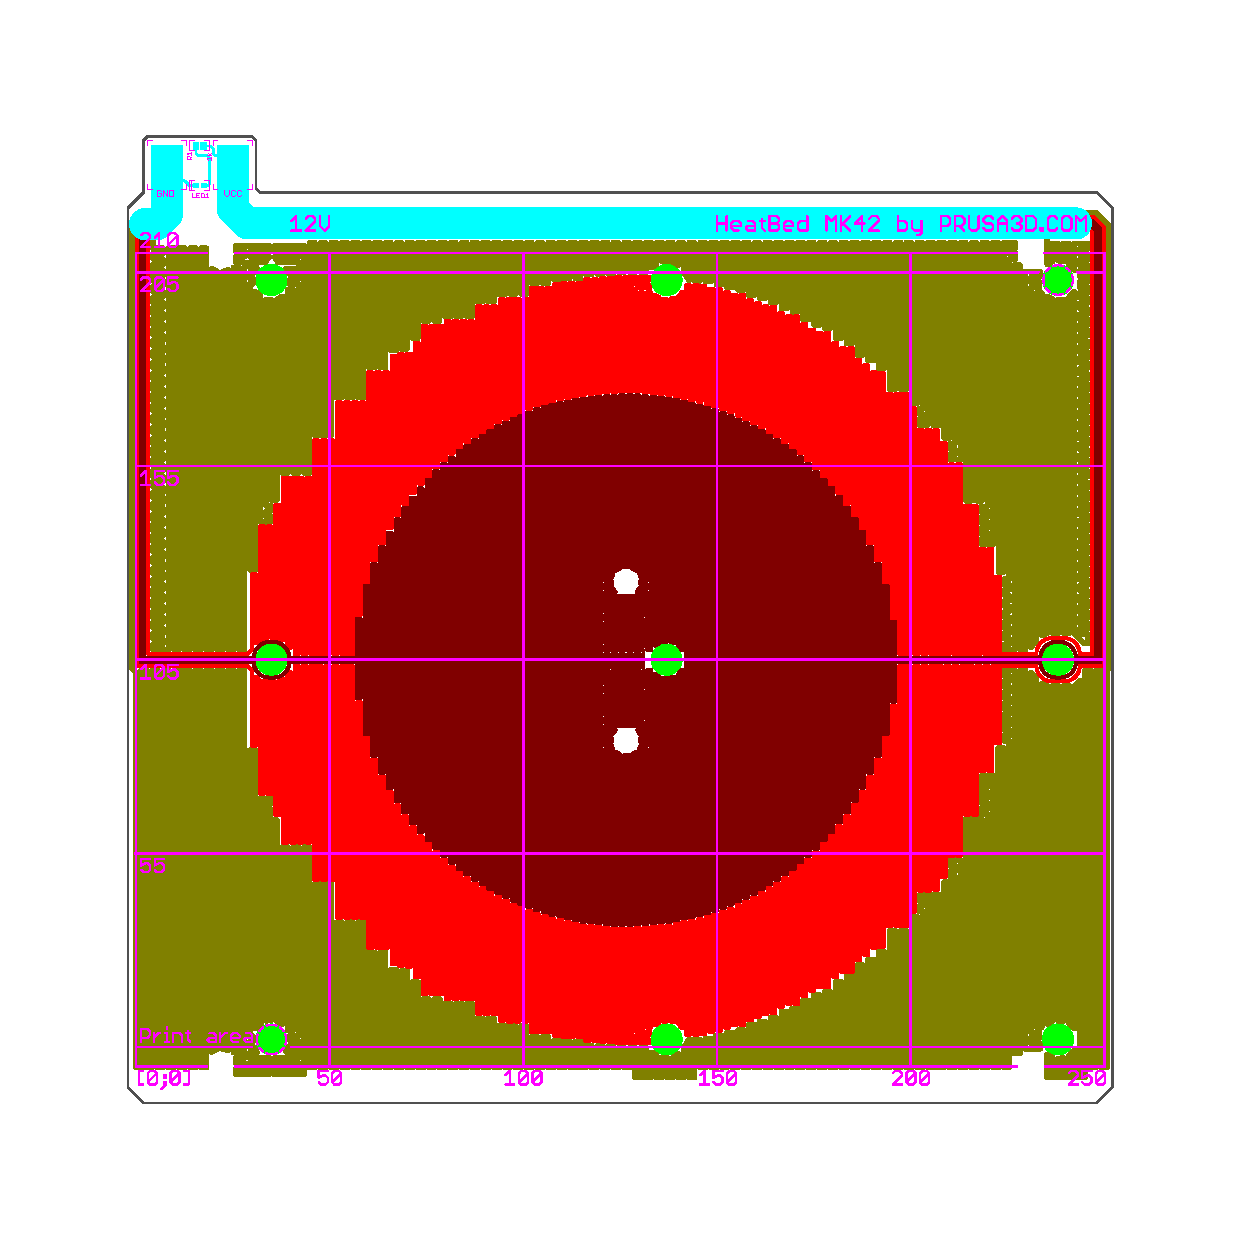
\includegraphics[width=1.0\textwidth, trim = 50px 50px 50px 50px, clip]{./bilder/MK42Bed.pdf}
\end{framed}

\end{minipage}}
\hfill
\adjustbox{valign=t}{\begin{minipage}[t]{0.60\textwidth}
\vspace{0pt}
\subsection{MK42}
\huge
Das MK42 hat 3 verschiedene Heizzonen.\\
Dadurch ist die Oberfläche gleichmäßig beheizt.
Es verfügt über 9 Kalibrierungspunkte welche eine X Y Z Autokalibrierung ermöglichen.
% \caption{Kapazität}
\end{minipage}}
\end{figure}

\clearpage % GleitObjekte anzeigen

\newpage % ============================================= Newpage ===================

\section{Hotend und Extruder}
\begin{center}
  Es gibt 2 Arten von Hotend / Extruder Setups ...
\end{center}

% \begin{framed}

% \end{framed}
\begin{center}
  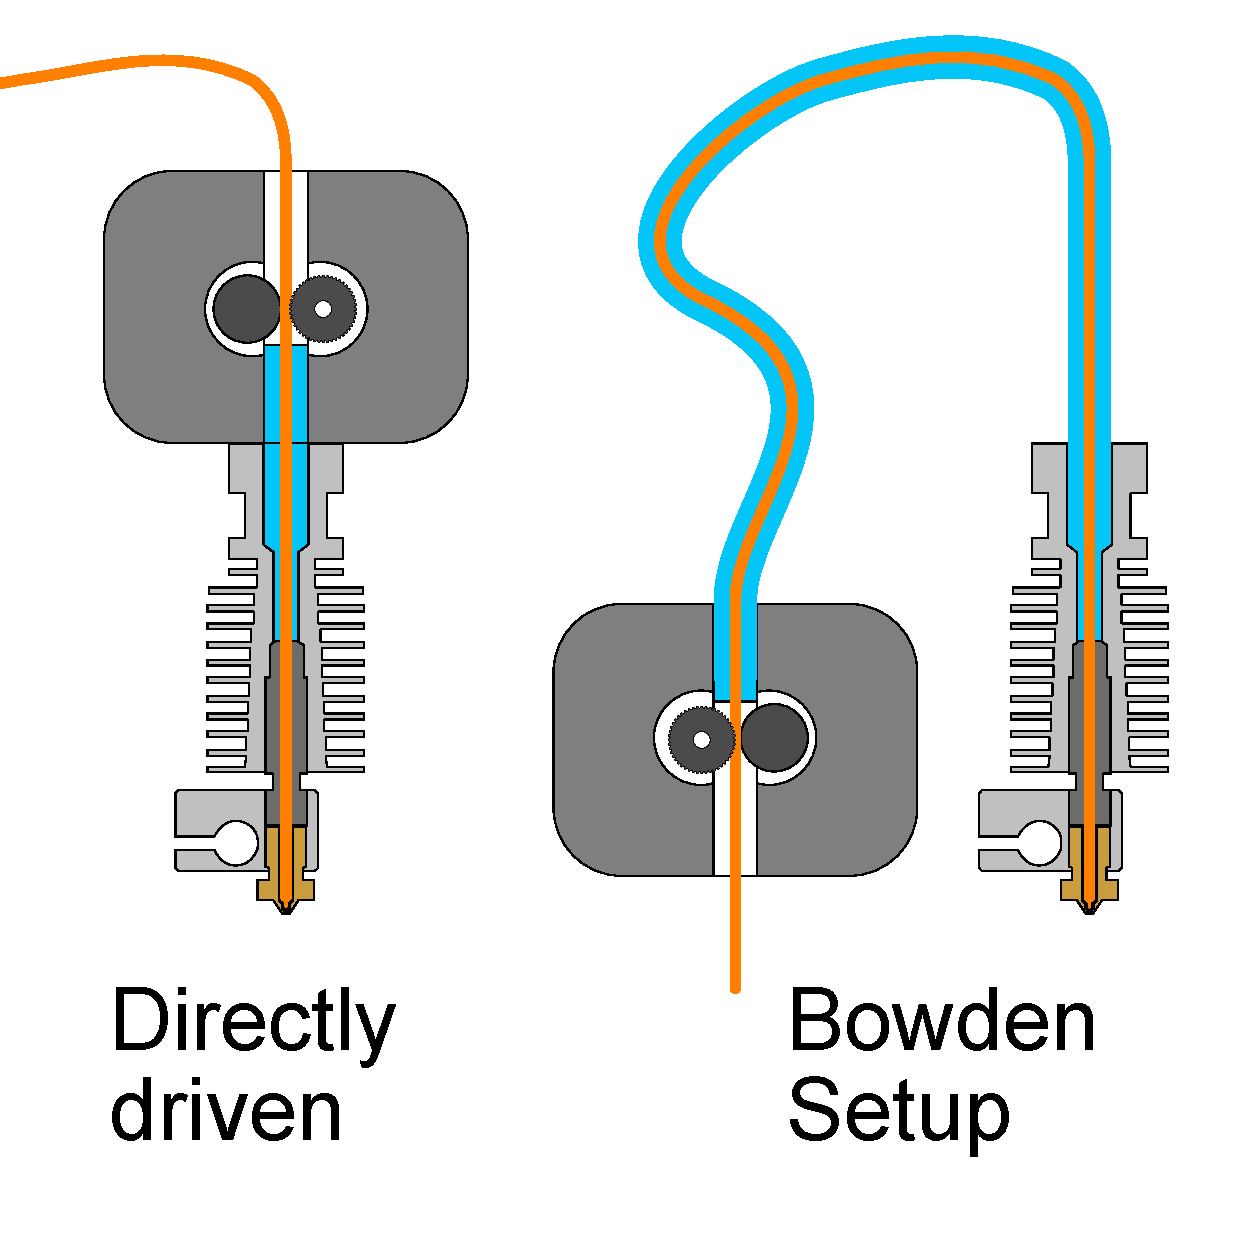
\includegraphics[scale=0.6]{./bilder/Extruder.pdf}
\end{center}

\newpage % ============================================= Newpage ===================

\section{Ein Delta ohne Riemen}
\vspace{1cm}
\begin{center}
  Ein Drucker ohne Zahnriemen in Delta-Bauweise ist sehr gut umsetzbar.
\end{center}
\vspace{1cm}
\begin{itemize}
  \item Es müssen keine Bänder nachgespannt werden
  \item Kein \"{} Spiel \"{} zwischen den Riemen und den Antriebsrädern.
  \item Durch direkten Antrieb und einer Übersetzung ist eine hohe \\ Geschwindigkeit bei gleichzeitig hoher Präzision möglich.
  \item Bei einem Delta spart man generell einen Motor
\end{itemize}

\newpage % ============================================= Newpage ===================

\subsection{Der Drucker in der Ausgangsstellung}
\begin{center}
  Alle Endschalter lösen aus. \\Der Drucker hat den Druckkopf ganz nach oben gefahren.
\end{center}

% \begin{framed}

% \end{framed}
\begin{center}
  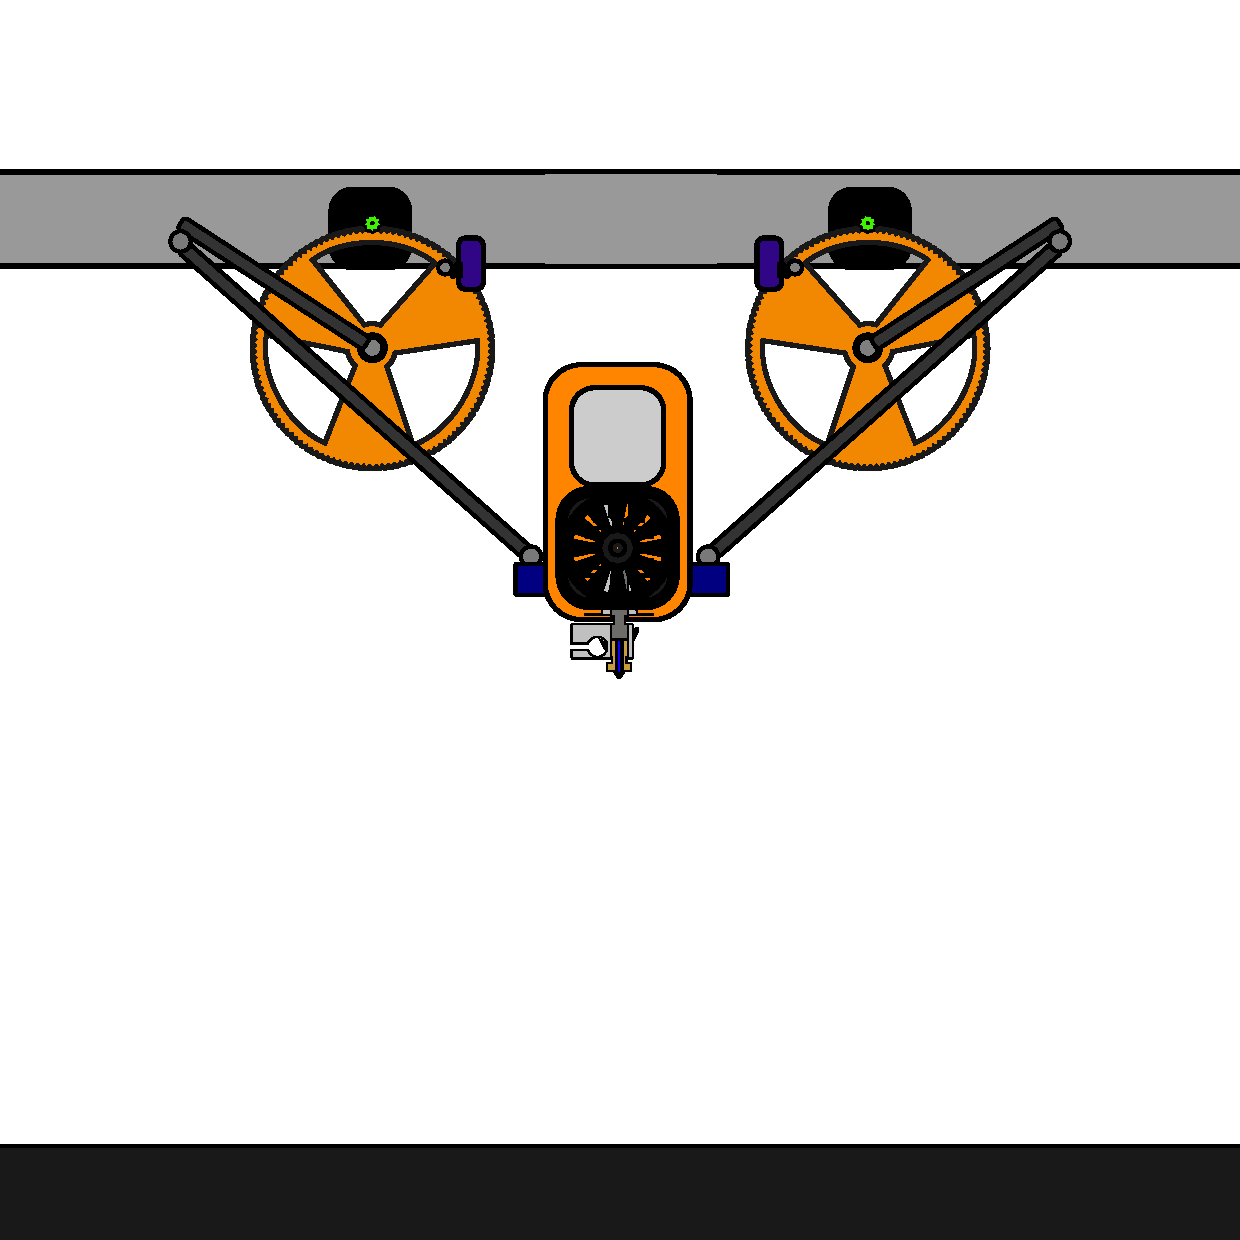
\includegraphics[scale=0.5]{./bilder/mydelta.pdf}
\end{center}

\newpage % ============================================= Newpage ===================

\subsection{Drucker mit abgesenktem Hotend}
% \begin{center}
%   Es gibt 2 Arten von Hotend / Extruder Setups ...
% \end{center}

% \begin{framed}

% \end{framed}
\begin{center}
  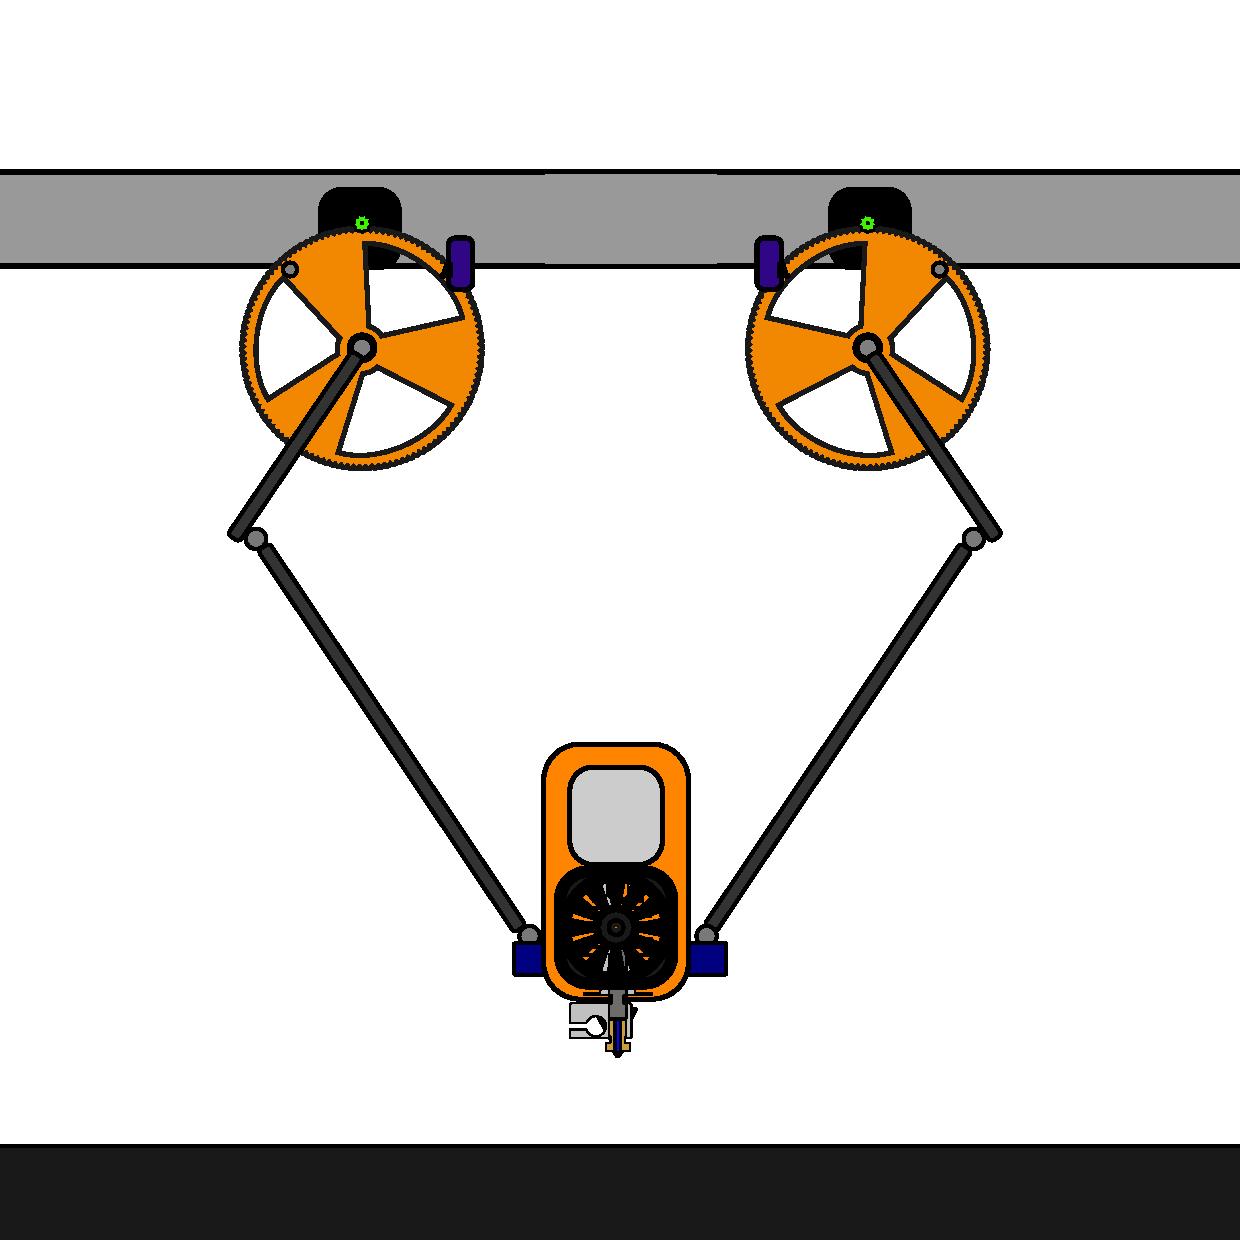
\includegraphics[scale=0.6]{./bilder/mydeltaDown.pdf}
\end{center}

\newpage % ============================================= Newpage ===================

\subsection{Drucker mit nach links gefahrenen Druckkopf }
% \begin{center}
%   Es gibt 2 Arten von Hotend / Extruder Setups ...
% \end{center}

% \begin{framed}

% \end{framed}
\begin{center}
  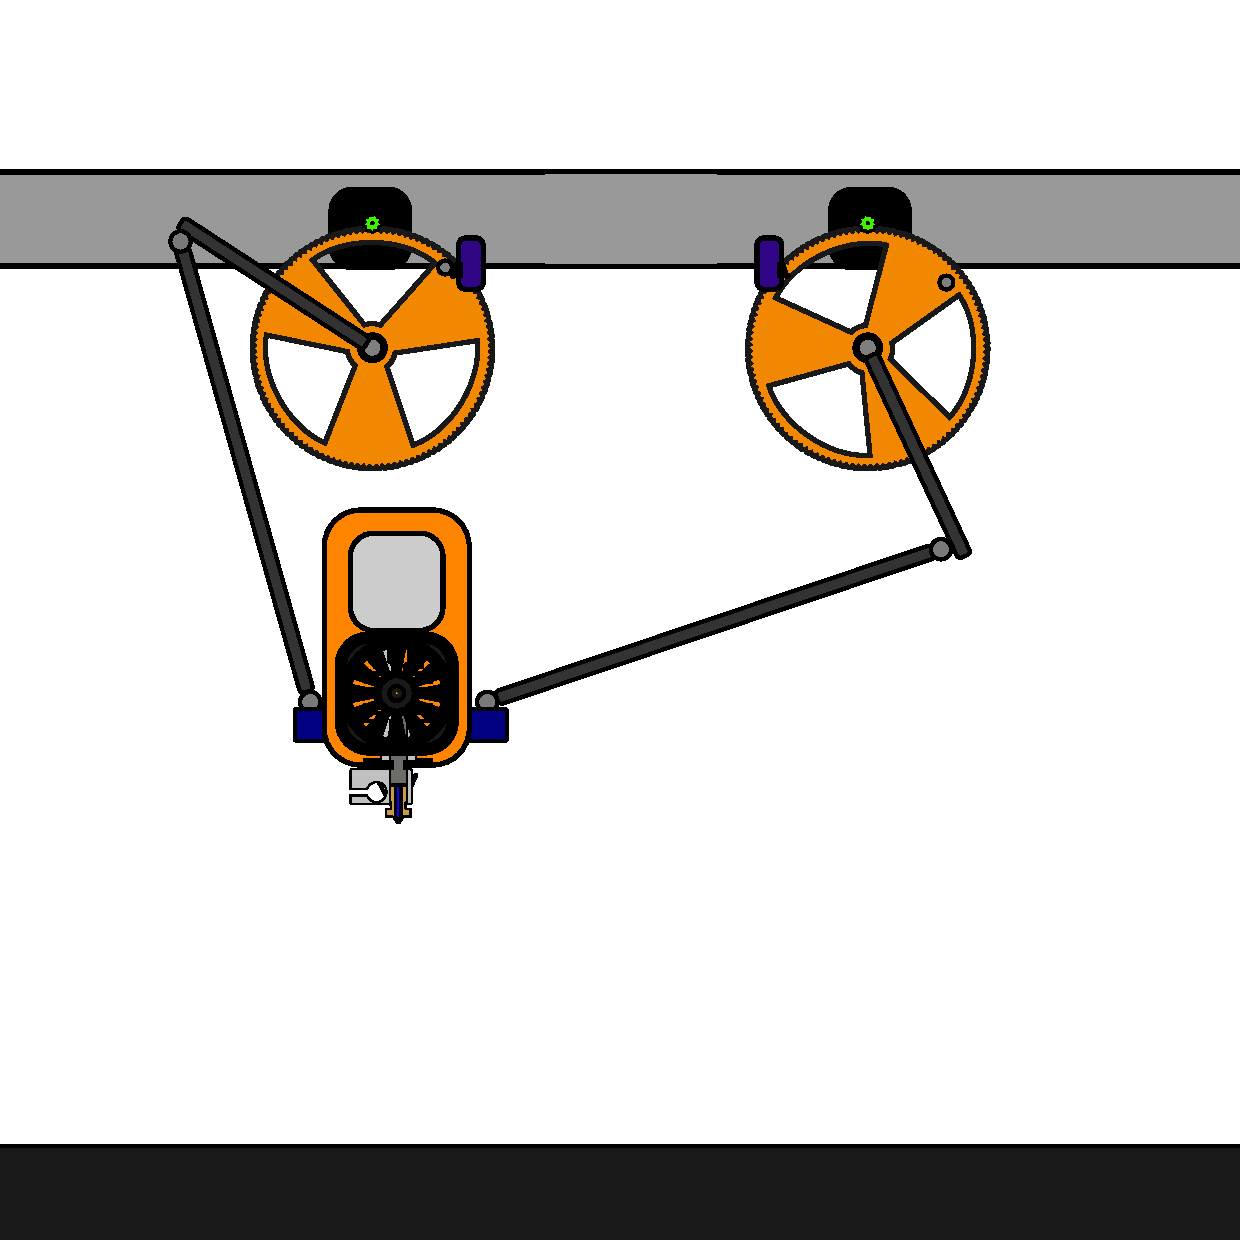
\includegraphics[scale=0.6]{./bilder/mydeltaleft.pdf}
\end{center}
